\documentclass[crop,tikz]{standalone}

\usetikzlibrary{calc}
\usetikzlibrary{arrows}
\usetikzlibrary{arrows.meta}

\begin{document}
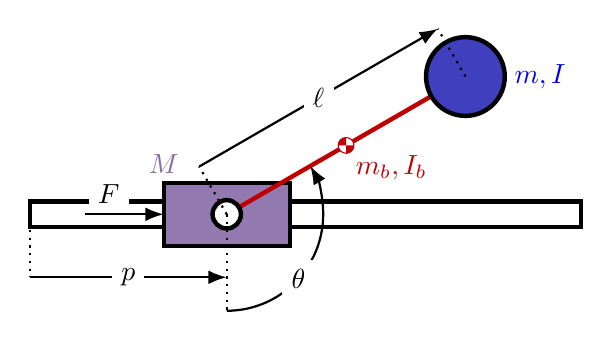
\begin{tikzpicture}

\colorlet{rodcolor}{red!75!black}

\colorlet{diskcolor}{blue!50!gray}
\colorlet{diskcolorcontour}{blue!0!black}
\colorlet{diskcolortext}{blue!90!black}

\definecolor{mypurple}{RGB}{146, 121, 176}
\colorlet{masscolor}{mypurple}
\colorlet{masscolorcontour}{mypurple!0!black}
\colorlet{masscolortext}{mypurple!90!black}

\def\quadwidth{0.8}
\def\quadheight{0.4}
\def\jointrad{0.18}

\def\phiangle{30}
\def\rodlen{3.5}
\def\diskrad{0.5}

\coordinate (diskDir) at ({cos(\phiangle)}, {sin(\phiangle)});
\coordinate (diskOrt) at ({-sin(\phiangle)}, {cos(\phiangle)});
\coordinate (diskPos) at ($\rodlen*(diskDir)$);

% DRAW THE RAIL
%  \def\raillen{2.0}
%  \def\railoffs{0.5}
\def\raillen{3.5}
\def\railoffs{-1.0}
\def\railheight{{0.4*\quadheight}}
\draw[ultra thick] ({-\raillen-\railoffs},{-\railheight}) rectangle (\raillen-\railoffs,\railheight);

% DRAW THE BASE
\filldraw[ultra thick,draw=masscolorcontour,fill=masscolor] (-\quadwidth,-\quadheight) rectangle (\quadwidth,\quadheight);
\node[above,masscolortext] () at ({-\quadwidth},{\quadheight}) {$M$};

% DRAW THE ROD
\draw[ultra thick,rodcolor] ($\jointrad*(diskDir)$) -- ($(diskPos)-\diskrad*(diskDir)$);

% DRAW THE "COM" SYMBOL
\def\comradius{0.1}
\fill[white] ($0.5*(diskPos)$) circle (\comradius);
%  \fill[\rodcolor] ($0.5*(diskPos)$) -- ++({\comradius},0) arc [start angle=0,end angle=90,radius={\comradius}] -- ++(0,{-\comradius});
%  \fill[\rodcolor] ($0.5*(diskPos)$) -- ++({-\comradius},0) arc [start angle=180,end angle=270,radius={\comradius}] -- ++(0,{\comradius});
\fill[rodcolor] ($0.5*(diskPos)$) -- ++(0,{\comradius}) arc [start angle=90,end angle=180,radius={\comradius}] -- ++({\comradius},0);
\fill[rodcolor] ($0.5*(diskPos)$) -- ++(0,{-\comradius}) arc [start angle=270,end angle=360,radius={\comradius}] -- ++({-\comradius},0);
\draw[rodcolor] ($0.5*(diskPos)$) circle (\comradius) node[below right] {$m_b,I_b$};

% DRAW THE PIVOT JOINT
\filldraw[ultra thick,draw=black,fill=white] (0,0) circle (\jointrad);

% DRAW THE DISK
\filldraw[ultra thick,draw=diskcolorcontour,fill=diskcolor] (diskPos) circle (\diskrad);
\node[right,diskcolortext] () at ($(diskPos)+(\diskrad,0)$) {$m,I$};


% DRAW THE LENGTH "ell" OF THE ROD
\def\rodortlen{0.7}
\draw[dotted,thick] (0,0) -- ($\rodortlen*(diskOrt)$);
\draw[dotted,thick] (diskPos) -- ($(diskPos)+\rodortlen*(diskOrt)$);
\draw[-Latex,thick] ($\rodortlen*(diskOrt)$) -- ($(diskPos)+\rodortlen*(diskOrt)$) node[midway,fill=white](){$\ell$};




\def\phiarcfrac{0.35}
\draw[dotted,thick] let \p1=(diskPos) in (0,0) -- (0, {-\phiarcfrac*\rodlen});
\draw[-Latex, thick] (0,{-\phiarcfrac*\rodlen}) arc (-90:\phiangle:{\phiarcfrac*\rodlen}) node[pos=0.4,fill=white](phiText) {$\theta$};

\def\refoffset{0.8}
\def\posorigin{{-\raillen-\railoffs}}
\draw[dotted, thick] ({\posorigin},0) -- ({\posorigin},{-\refoffset});
\draw[-Latex, thick] ({\posorigin},{-\refoffset}) -- (0,{-\refoffset}) node[midway,fill=white] (posText) {$p$};


\def\forcelen{1.0}
%  \draw[-Latex,thick, blue] ({-\forcelen-\quadwidth},0) -- ({-\quadwidth},0) node[pos=0.3,above,fill=white,text=black](){\color{blue}$f$};
\draw[-Latex,thick] ({-\forcelen-\quadwidth},0) -- ({-\quadwidth},0) node[pos=0.3,above,fill=white](){$F$};

\end{tikzpicture}
\end{document}